\documentclass{pset}

\usepackage{graphicx}

\newcommand{\widevec}[1]{\overrightarrow{#1}}

\psnum{5k}
\date{Due Thursday, April 17}
\versionnumber{2}


\begin{document}
\maketitle{}

\section*{Karma apps}

We have provided you some extra apps to implement if you want to play with your
MapReduce implementation to do some interesting things.

\begin{note}{Note}
To add a new app, you should edit \filename{apps/appList.ml} and include your
app's module.  In addition, you should edit the file \filename{.depend} in the
\filename{release} directory and add the directory containing your app.
\end{note}

\part{N-body simulation}
If one has $n$ physical bodies moving in empty space, each one will exert a
gravitational force on each of the others.  This will cause the objects to move
over time, which in turn will change the forces acting on each object.

An $n$-body simulation models this situation by repeatedly computing the force
on an object and then moving the objects over a small time span.

This kind of simulation is a natural fit for the MapReduce framework: the forces
between each pair of objects can be computed completely independently of all of
the other pairs, and can thus happen in parallel.

To simulate a moving object, we need to know its position, mass, and
velocity.
\begin{ocaml}
type body = {
  mass     : Vector.scalar;
  location : Vector.t;
  velocity : Vector.t;
}
\end{ocaml}

Given this information, we can compute the force that one body exerts on
another, and from this, we can compute the acceleration on $x$:

\begin{displaymath}
\widevec{a_{xy}} = \frac{G \cdot mass_y}{||\widevec{d}||^3} \widevec{d}
\qquad \textrm{where } \widevec{d} = \widevec{pos_x} - \widevec{pos_y}
\end{displaymath}

The total acceleration on a body $x$ is just the sum of all of the accelerations
caused by the other bodies.  Using this, we can compute the new position and
velocity of $x$ after a short time $dt$:

\begin{displaymath}
\widevec{newpos_x} = \widevec{pos_x} + \widevec{v_x} \cdot dt + \frac{\widevec{a} \cdot dt^2}{2}
\qquad
\widevec{newv_x} = \widevec{v_x} + \widevec{a} \cdot dt
\end{displaymath}

Given a collection of bodies, we can use a single MapReduce job to compute the
updated bodies: the map phase can compute the acceleration for each pair of
bodies, and the reduce phase can combine all of these accelerations for a single
body to compute the new position and velocity.  We can then repeatedly execute
this job to simulate the bodies over a long time period.

We have provided you with some starter code to implement an $n$-body
simulation.  The \code{Vector} module is a convenient way to
manipulate vectors.
  The \code{Simulations} module has routines for reading initial
configurations and outputting transcripts.
What's left for you to implement is the \code{Nbody.Job} module and the
\code{run} function that will use it to compute the output.

\begin{figure}
\begin{center}
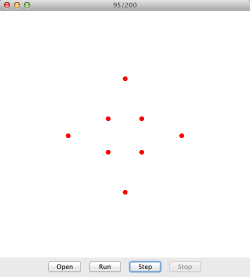
\includegraphics{nbody-gui.png}
\end{center}
\caption{The \code{bouncy.jar} gui.}
\label{fig:bouncy}
\end{figure}


The transcripts output by \code{Simulations.write_transcript} can be read by
the program \filename{bouncy.jar}, which displays a nice animation (see
figure~\ref{fig:bouncy}):

\begin{ocaml}
% cs3110 run controllerMain.ml -local nbody apps/nbody/data/zardoz.bodies 300 out.txt
% java -jar bouncy.jar out.txt
\end{ocaml}

\newpage{}
\part{Web search}

The original motivating example for MapReduce was web search.  We have provided
you with some infrastructure for building a fully featured web search tool.

The first part of searching the web involves crawling the web to find pages to
search.  We have provided you with a MapReduce job that does just that: the
function \code{Crawler.crawl} takes a starting list of pages, and
a desired number of pages $n$, and follows links from the
starting pages until it has fetched $n$ pages.

\begin{note}{Note} the crawler depends on an the opam libraries
\filename{cohttp} and \filename{ocamlnet}.  To run it, you will
need to install them:
\begin{ocaml}
opam install cohttp ocamlnet
\end{ocaml}
You will also need to add the following lines to the
\filename{.opam\_packages} file in the \filename{release/}
directory
\begin{ocaml}
cohttp.async
netstring
\end{ocaml}
\end{note}

\exercise{Extend word count to the web}

Using the crawler, implement the \code{WebCount} app, which extends the
\code{WordCount} module to work on web pages instead of files.

\begin{ocaml}
% cs3110 run controllerMain.ml webcount -local 200 http://www.cnn.com/
$\cdots$
found 4216 pages, returning 4216 of them
$\cdots$
"cnn":          716
"{":            834
"on":           864
"for":          914
"}":            1045
"in":           1329
"|":            1399
"and":          1480
"a":            1632
"of":           1675
"to":           2061
"the":          3485

total words: 129799
\end{ocaml}


\exercise{Implement web search}

The provided \code{Ocoogle} app uses the crawler to fetch web pages, and then
invokes \code{PageRank.page_rank} function to rank the results,
and then repeatedly prompts the user for a search term and calls
\code{Search.search} to find a list of pages to return.

In the release code, the \code{Search.search} function doesn't work very well
--- it simply returns the first 9 pages, without considering the user's query
or the page rankings.  Using one or more MapReduce jobs, make it return the top
10 ranked pages that are relevant to the query.

\begin{note}{Hint} To find the top 10 results, you can randomly divide all of
the results into $n$ buckets; if you have the top ten results from each bucket,
you are guaranteed that the overall top ten are within the $10n$ results
returned.
\end{note}

\begin{ocaml}
% cs3110 run controllerMain.ml webcount -local 200 http://www.cnn.com/
$\cdots$
enter a search string (or control-D to exit)
post
(#1) breaking news and opinion on the huffington post
      http://www.huffingtonpost.com?hpt=hp_bn8

(#2) udonis haslem breaks down his for guarding players in the post $\cdots$
      http://bleacherreport.com/articles/2025091-udonis-haslem-$\cdots$

(#3) your facebook news feed is about to get a lot less annoying
      http://www.huffingtonpost.com/2014/04/10/facebook-newsfeed-$\cdots$


enter a search string (or control-D to exit)
facebook
(#1) your facebook news feed is about to get a lot less annoying
      http://www.huffingtonpost.com/2014/04/10/facebook-newsfeed-$\cdots$

enter a search string (or control-D to exit)
money
(#1) cnnmoney - business financial and personal finance news
      http://money.cnn.com/?cnn=yes

$\cdots$
\end{ocaml}


\exercise{Implement Page Rank}

In the release code, the \code{PageRank.page_rank} function also doesn't work
very well --- it gives every page the same rank.

Many search engines use a variant of an algorithm called PageRank (named after
Larry Page, who invented the algorithm and founded Google).  The idea behind
Page Rank is that when one page links to another, it can be interpreted as a
statement by the linking page that the linked page is useful.  This means that
if you start at a random page and randomly follow links, you are likely to end
up on a useful page.

This probability can be estimated as follows.  Begin by assigning the same
weight to every page ($1/n$ where there are $n$ pages to rank).  Then perform a
number of rounds; in each round, each page's weight gets distributed evenly
among all of the pages it links to.  These weights are then summed, with small
adjustments to account for the probability that a user stays on a given page,
or jumps to another page randomly.

The formula for the rank of page $p$ in the $i+1$st round is given by:
\begin{displaymath}
rank_{p,i+1} = bonus_i + \sum_{\textrm{pages $p'$ that link to $p$}} d \frac{rank_{p',i}}{\textrm{\# links out of }p'}
\end{displaymath}
where $d$ is a damping factor (to account for the probability that a user stays
on the same page; $.85$ is a typical value), and $bonus_i$
accounts for pages that don't link anywhere (sinks):
\begin{displaymath}
bonus_i = \frac{1 - d\sum_{p \in Sinks}(1 - rank_{p,i})}{n}
\end{displaymath}

This process is repeated until the probabilities stop changing significantly;
10 repetitions typically gives pretty good results.

For more discussion of the PageRank algorithm, see the
\link{http://en.wikipedia.org/wiki/PageRank}{Wikipedia page on
PageRank}.

PageRank fits naturally into the MapReduce framework: each round can be executed
as a MapReduce job; the map phase of this job outputs the contribution of a page
to each page that it links to, and the reduce phase can weight and sum these
contributions to calculate the rank of the page at the end of the round.

\end{document}
